\documentclass{article}

\usepackage[OT1]{fontenc}
\usepackage{mathpazo}
\usepackage[italian]{babel}

%math
\usepackage{amsmath}
\usepackage{amssymb}
\usepackage{amsfonts}
\usepackage[utf8]{inputenc}
\usepackage{cancel}

%Graphics&Float
\usepackage{graphicx}
\usepackage{float}

%Hypelinks
\usepackage{hyperref}
\hypersetup{
    colorlinks,
    citecolor=black,
    filecolor=black,
    linkcolor=black,
    urlcolor=black
}

% TIKZ
\usepackage{tikz}
\usetikzlibrary{shapes.geometric, arrows}
\tikzstyle{arrow} = [thick,->,>=stealth]
\tikzstyle{startstop} = [rectangle, rounded corners, minimum width=3cm, minimum height=1cm,text centered, draw=black, fill=red!30]
\tikzstyle{io} = [trapezium, trapezium left angle=70, trapezium right angle=110, minimum width=3cm, minimum height=1cm, text centered, draw=black, fill=blue!30]
\tikzstyle{process} = [rectangle, minimum width=3cm, minimum height=1cm, text centered, draw=black, fill=orange!30]
\tikzstyle{decision} = [diamond, minimum width=3cm, minimum height=1cm, text centered, draw=black, fill=green!30]

%Algorithm
\usepackage[]{algorithm2e}

\title{\textbf{Informatica Teorica}}
\author{Manuel Pagliuca}

\begin{document}
\maketitle
\tableofcontents
\pagebreak
\section{Introduzione}
Nei corsi di informatica applicata come quelli di: Sistemi Operativi, Basi di dati, ecc... l'oggetto di studio è definito dal corso, e l'informatica è lo strumento per studiare questo oggetto.

Nel corso di informatica teorica l'oggetto di studio è l'informatica stessa, si studiano i fondamenti dell'informatica (come un corso di sistemi operativi effettua uno studio sui fondamenti dei sistemi operativi).

Per eseguire lo studio di questa disciplina ci si pone le due domande fondamentali nei confronti dell'informatica \textit{cosa} e \textit{come}.
\subsection{Cosa studia l'informatica?}
L'informatica è una disciplina che studia l'informazione e l'elaborazione automatica mediante sistemi di calcolo che eseguono programmi.

Ma sappiamo che tutti i problemi sono risolubili per via automatica, e questo porta proprio alla nostra domanda, quali problemi sono in grado di risolvere \textit{automaticamente}?

Ciò che studia il \textit{cosa} dell'informatica si chiama \textbf{teoria della calcolabilità}, mostreremo nelle successive lezioni che non è una domanda cosi facile da rispondere, poichè esistono delle cose che non sono calcolabili. Quindi dato che non ci sono cose calcolabili, la teoria della calcolabilità si domanda \textit{che cosa è calcolabile?}.
\newline
Nella teoria della calcolabilità vogliamo una risposta generale, non cerchiamo dei casi particolari per dire questo è calcolabile o meno, esistono delle proprietà che accomunano tutto ciò che è calcolabile ? La risposta è si, la nozione di calcolabilità è denotabile attraverso la matematica e quindi posso affrontare l'insieme di cose fattibili dell'informatica con gli strumenti della matematica.
\subsection{Come l'informatica risolve i problemi?}
La branca dell'informatica che si chiama \textbf{teoria della complessità} risponde alla domanda \textit{come è risolubile questo problema ?}. Essa studia la quantità di risorse computazionali richieste dalla \textit{soluzione automatica} dei problemi. Una \textit{risorsa computazionale} è qualsiasi cosa venga sprecata per l'esecuzione dei programmi:

Le principali risorse su cui ci concentreremo sono il \textbf{tempo} e \textbf{spazio di memoria}, dovremo quindi dare una definizione rigorosa di queste risorse computazionali. Successivamente si potrà porre delle domande ovvie : \textit{quale è la classe di problemi che vengono risolti efficientemente in termini di tempo e di memoria ?}. Notare che nella teoria della complessità non si parla solo di \textbf{risolubilità} (come nella teoria della calcolabilità) ma anche dell'\textbf{efficienza} con cui risolvo questo problema.
\newline
Esistono problemi che si trovano in una zona grigia, che non sappiamo se hanno una risoluzione efficiente, ma sono problemi molto importanti, nessuno è riuscito a dimostrare se avranno soluzioni efficienti ma nemmeno il contrario, ovvero nessuno è riuscito a dimostrare che saranno risolubili efficientemente. Questa classe di problemi è la classe di problemi NP, vedremo poi di cosa si tratta.
\section{Syllabus}

\begin{itemize}
    \item Teoria della calcolabilità: individuare la qualità della calcolabilità dei problemi, quali sono le categorie di problemi calcolabili e distinguerla da quella dei problemi non calcolabili.
    \item Teoria della complessità: studio quantitativo dei problemi, dopo aver delimitato il confini di ciò che è calcolabile cercare un sotto insieme di problemi \textbf{efficientemente calcolabili}.
\end{itemize}

\pagebreak
\section{Il nostro linguaggio: la matematica}
\subsection{Funzione}
Una funzione dall'insieme $A$ all'insieme $B$ è una \textbf{legge}, che chiamiamo solitamente $f$, che spiega come associare ad ogni elemento di $A$ un elemento di $B$.
\newline

Dal punto di vista formale l'espressione della funzione viene definita \textbf{globalmente}:
$$f:A\rightarrow B$$
Dove $A$ viene chiamato \textbf{dominio} e $B$ \textbf{codominio}, questa notazione dice che ogni elemento del dominio è associato attraverso una legge $f$ ad un elemento del codominio. Esiste anche uan notazione che permette di stabilire localmente l'operato della funzione, essa rappresenta l'operato della legge $f$ sull'elemento $a$ che porta all'elemento $b$.
$$a \xrightarrow[\text{}]{\text{f}} b$$
\newline
La notazione comunemente più utilizzata (in particolare nei libri di testo, ma anche nei corsi di matematica), è la seguente:
$$f(a)=b$$
Solitamente $b$ è l'\textbf{immagine} di $a$ secondo $f$, e meno usualmente si dice che $a$ è la \textbf{controimmagine} di $b$ (sempre secondo $f$).
\newline
\newline
Per esempio:
$$f:\mathbb{N} \rightarrow \mathbb{N}$$
Dove $\mathbb{N}$ è l'insieme dei numberi naturali ${0,1,2,3,...}$, e per utilizzi futuri denotiamo con $\mathbb{N}^+$ l'insieme dei numeri naturali positivi (zero escluso) ${1,2,3,4,...}$.
\newline
Ora vediamo la specifica della funzione $f$
$$f(n)=\lfloor \sqrtsign{n}\rfloor$$
Considerando $n=5$ l'immagine di quest'ultima sarà $f(5)=\rfloor\sqrt{5}\lfloor=2$.
\newline
Quindi possiamo dedurre che per più elementi del dominio una \textbf{funzione} effettua un mapping ad uno ed un solo valore del codominio (nel caso in cui un valore del dominio venga mappato a più valori del codominio allora si parla di relazione, ma non più di funzione).
\subsection{Classi di funzioni}
\subsubsection{Funzioni iniettive}

Una funzione è \textbf{iniettiva} se e solo se elementi diversi del dominio vengono mappati in elementi diversi del codominio.
$$f:A\rightarrow B\text{ è iniettiva sse } \forall a_1,a_2\in A \text{ dove } a_1\neq a_2 \implies f(a_1)\neq f(a_2)$$
\newline
\textit{Esempio 1}
$$f(n)=\lfloor\sqrt(n)\rfloor$$
Abbiamo visto precedentemente che questa funzione non è iniettiva, perché avviene un mapping per più elementi del dominio ad un unico elemento del codominio.
\newline
\newline
\textit{Esempio 2}
$$f(n)=[n]_2$$
Questa funzione è fortemente non iniettiva, le due metà dell'insieme dei numeri naturali vengono mappate solamente su due numeri $f(2k)=0$ e $f(2k+1)=1$.
\newline
\newline
\textit{Esempio 3}
$$f(n)=n^2$$
Questa è una funzione iniettiva, poiché ad ogni controimmagine corrisponde una immagine distinta.

\subsubsection{Funzioni suriettive}
Una funzione è suriettiva quando tutti gli elementi del codominio hanno una corrispondenza con un elemento del dominio.
$$f:A\implies B\text{ sse } \forall b\in B, \exists a \in A : f(a)=b$$
\noindent
\textit{Esempio 1}
\newline
$f(n)=\lfloor\sqrt{n}\rfloor$ è suriettiva, questo perchè $\forall m\in \mathbb{N}, m=\lfloor\sqrt{m^2}\rfloor=f(m^2)$. Sostanzialmente, posso tornare con facilità al dominio perchè mi basta elevare al quadrato l'immagine, e questo è fattibile per tutto l'insieme dei numeri naturali.
\noindent
\newline
\linebreak
\textit{Esempio 2}
\newline
$f(n)=[n]_2$ non è una funzione suriettiva, questo perchè per esempio $3$ non è immagine di niente rispetto a $f$ (il codominio è tutto $\mathbb{n}$).

\subsection{Insieme immagine di una funzione}
$$Im_f={b\in B:\exists a,f(a)=b}={f(a):a\in A}$$

Data $f$ definitiamo l'\textbf{insieme immagine di $f$} come gli elementi del codominio $\in B$ che sono immagine di un elemento del dominio $A$.
\newline
La relazione tra questo insieme $Im_f$ ed il codominio stesso di $f$ quale è $B$, consiste in:
$$Im_f\subseteq B$$
Allora possiamo dire che una funzione è suriettiva quando:
$$Im_f=B$$
\newline
\textit{Esempi}
$$Im_{\lfloor\sqrt{n}\rfloor}=\mathbb{N}\implies f(n)=\lfloor\sqrt{n}\rfloor \text{ è suriettiva}$$
$$Im_{[n]_2}={0,1}\subseteq \mathbb{N} \implies f(n)=[n]_2 \text{ non è suriettiva}$$

\subsection{Funzioni biettive}
Una funzione si dice biettiva quando è sia suriettiva che iniettiva, devono valere entrambe le due condizioni (questo due condizioni è possibile fonderle in un unica condizione).
$$f:A\rightarrow B \textbf{ sse }$$
$$\forall a_1,a_2 \in A, a_1\neq a_2 \implies f(a_1)\neq f(a_2) \land \forall b\in B, \exists a\in A:f(a)=b$$
Che converge in un unica definizione:
$$\forall b \in B,\exists !a\in A : f(a)=b$$
Per esempio: $f(n)=n$, oppure considerando gli insiemi dei numeri reali $f(x)=x^3$. Solo per questa tipologia di funzioni esiste il concetto di \textbf{funzione inversa}.

\subsection{Inversa di una funzione}
Data una funzione $f$ biettiva si definisce l'inversa come $f^{-1}$ la funzione tale che crei un mapping tra l'immagine del codominio rispetto alla controimmagine del dominio.
$$f:A\rightarrow B$$
$$f^{-1}:B\rightarrow A \text{ tale che } f^{-1}(b)=a \Longleftrightarrow (a)=b$$

Per esempio l'inversa di $f(n)$ è $f^{-1}=n$, oppure l'inversa di $f(x)=x^3$ è $f^{-1}=\sqrt[3]{x}$ (considerando l'insieme dei numeri reali).

\subsection{Composizione di funzioni}
Date due funzioni $f:A\rightarrow B$ e $g:B\rightarrow C$, notiamo che queste funzioni hanno una caratteristica in comune, ovvero che il codominio di una è il dominio dell'altra.
Definiamo la composizione di funzione $g\circ f:A\rightarrow C$ come la funzione che va da dal dominio di $f$ al codominio di $g$, definita come $g(f(a))$.
$$g\circ f=g(f(a))$$

Per esempio $f(n)=n+1 \text{ e } g(n)=n^2$:
\begin{itemize}
    \item $f \text{ composto } g: g\circ f(n)=(n+1)^2$
    \item $g \text{ composto } f: f\circ g(n)=n^2+1$
\end{itemize}

N.B. L'operazione di composizione restituisce una funzione, e l'operatore $\circ$ non è commutativo, però quando dominio e codominio lo permettono è \textbf{associativo}: $(f\circ g)\circ h=f\circ (g \circ h)$.

\subsubsection{Funzione identità}
La funzione identità sull'insieme $A$ è una funzione che effettua un mappaggio ricorsivo sullo stesso elemento.
$$i_A:A\rightarrow A : i_A(a)=a\text{ }\forall a\in A$$
Per esempio la funzione identità sull'insieme $\mathbb{N}$ è $i_\mathbb{N}(n)=n$.

\subsubsection{Definizione alternativa di funzione inversa}
Data una funzione $f:A\rightarrow B$ biettiva, la sua inversa è l'unica funzione $f^{-1}:B\rightarrow A$ che soddisfa:
$$f^{-1}(b)=a \longleftrightarrow f(a)=b$$
$$oppure$$
$$f^{-1}\circ f=i_A \land f\circ f^{-1}=i_B$$

Infatti considerando $f^{-1}\circ f(x) = \sqrt[3]{x^3}=x=i_\mathbb{N}(x)$ e $f\circ f^{-1}(x)=(\sqrt[3]{x})^3=x=i_\mathbb{N}(x)$

\subsubsection{Funzioni totali e parziali}
Considerando una funzione $f:A\rightarrow B$ essa è una legge che ad \textbf{ogni} elemento di $A$ si associa
un elemento di $B$, questo significa che ogni immagine $f(a)$ è definita per ogni elemento $a\in A$. Esiste
un apposita notazione:
$$f(a)\downarrow \forall a\in A$$

Una funzione di questo tipo viene chiamata \textbf{totale} poiché risulta definita sulla totalità del suo dominio.

Certe funzioni potrebbero \textit{non essere definita} per quale che elemento di $a\in A$, e quindi non avere delle immagini corrispondenti, la notazione:
$$f(a)\uparrow$$
Ovvero, che per un elemento $a$ non esiste immagine nell'insieme $B$ tramite la funzione $f$.

Consideriamo il seguente esempio:
$$f:\mathbb{N}\rightarrow\mathbb{N}$$
$$f(n)=\lfloor\frac{1}{n}\rfloor \text{ non è definita su } n=0\implies f(0)\uparrow \forall n\in\mathbb{N}\setminus{0}, f(n)\downarrow$$

Una funzione viene definita \textbf{parziale} se a \textit{qualche} elemento di $A$ si associa un elemento di $B$. Si amplia un nuovo concetto che è quello del \textbf{dominio} (o campo di esistenza) della funzione,
ovvero quell'insieme costituito da tutti gli elementi di $A$ tali per cui è definita una immagine appartenente a $B$.
$$Dom_f=\left\{a\in A : f(a)\downarrow \right\}\subseteq A$$

Allora vale precisare le due seguenti regole:
$$Dom_f\nsubseteq A\implies f\text{ parziale}$$
$$Dom_f\equiv A\implies f \text{ totale}$$

Alcuni esempi:
$$f(n)=\left\{\frac{1}{n}+\frac{1}{(n-1)(n-2)}\implies Dom_f=\mathbb{N}\setminus\{0,1,2\right\}$$
$$f(n)=\lfloor\log{n}\rfloor\implies Dom_f=\mathbb{N}\setminus\{0\}$$
$$f(n)=\lfloor\sqrt{-n} \implies Dom_f=\{0\}$$
\subsubsection{Totalizzazione di una funzione parziale}
Teniamo conto di una cosa, possiamo convenzionalmente rendere totale una funzione parziale, basta estendere
il codominio con un \textbf{simbolo convenzionale} $\bot$ che buttiamo fuori tutte le volte che la funzione non è definita.
$$f:A\rightarrow B\text{ parziale } \implies \widetilde{f}:A\rightarrow B\cap\{\bot\}$$
La totalizzazione di $f$ viene raggiunta con l'aggiunta di questo simbolo.
\[
    \widetilde{f}(a) =
    \begin{cases}
        f(a) & \quad\text{se }a\in Dom_f \\
        \bot & \quad\text{altrimenti}    \\
    \end{cases}
\]
Quindi per i punti dove il campo di esistenza non è definito verrà restituito $\bot$, per convenzione
quando una funzione parziale viene totalizzata ovvero $B\cap\bot$ possiamo utilizzare la seguente
notazione $B_{\bot}$.

\subsubsection{Prodotto cartesiano}
$$A\times B=\{(a,b):a\in A \land b\in B\}$$
Il \textbf{prodotto cartesiano} di due insiemi è l'insieme di coppie dove il primo elemento della coppia appartiene al primo insieme, ed il secondo elemento della coppia appartiene al secondo insieme.

Il prodotto cartesiano è un'operazione che non commuta.
$$A\times B \neq B\times A$$
Ovviamente l'unico caso dove un prodotto cartesiano è commutativo è quando $A\equiv B$.
Il prodotto cartesiano può essere esteso al prodotto di ennuple di più insiemi cartesiani,
dove questa volta il risultato è costituito da un insieme ordinato (non più di coppie) delle ennuple
rispettive agli insiemi di provenienza:
$$A_1\times A_2 \times ... \times A_n=\{(a_1,a_2,...,a_n):a_i\in A_i$$

Associato alla definizione di prodotto cartesiano abbiamo anche quella di \textbf{proiettore i'esimo},
essa è una funzione che agisce su un prodotto cartesiano. Ha come dominio l'insieme i-esimo di questo prodotto data una tupla del prodotto cartesiano non fa altro che estrapolare la componente i-esima di quella tupla (\textit{destruttura la tupla}).
$$\pi_i:A_1\times ...\times A_n\rightarrow A_i$$
$$\pi_i(a_1,...,a_n)=a_i$$
Utilizzeremo la seguente notazione esponenziale per calcolare il prodotto cartesiano di un insieme cartesiano
con se stesso:
$$A_1\times A_2\times A_3 ... \times A_n = A^n$$

Alcuni esempi:

$$C=\{(x,y)\in\mathbb{R}^2 : x^2+y_2=1\}\implies \text{ punti che si trovano lungo la circonferenza}$$
$$I=\{(x,y)\in\mathbb{R}^2 : x^2+y_2<1\}\implies \text{ punti che si trovano all'interno della circonferenza}$$
$$E=\{(x,y)\in\mathbb{R}^2 : x^2+y_2>1\}\implies \text{ punti che si trovano all'esterno della circonferenza}$$

$$C\cap I\cap E = \mathbb{R}^2$$

\subsubsection{Insieme di funzioni}
L'insieme delle funzioni che vanno dall'insieme $A$ a $B$ viene indicato con:
$$B^A=\{f:A\rightarrow B\} = \text{ insieme delle funzioni da } A \text{ a } B$$

L'insieme delle funzioni \textit{parziali} che vanno da $A$ a $B$:
$$B_{\bot}^A =\{f:A\rightarrow B_{\bot}\}=\text{ insieme delle funzioni parziali che va da A a B}$$

\subsubsection{Funzione di valutazione}
Dati due insiemi $A,B$ e $B_{\bot}^A$ si definisce una funzione di valutazione come:
$$\omega : B_{\bot}^A\times A \rightarrow B \text{ con } \omega (f,a)=f(a)$$
Essa è una funzione che valuta il punto del codominio $A$ in termini di $B$, ovvero restituisce un
$f(a)$, quindi il suo compito è strettamente quello di valutare.

\begin{itemize}
    \item Tenendo fisso $a$ e facendo variare $f$, è come se $a$ fosse un \textit{benchmark}
          su cui testiamo una serie di funzioni.
    \item Tenendo fisso $f$ e facendo variare $a$ ottengo il grafico di $f$.
\end{itemize}

\subsection{Modellare teoricamente un sistema di calcolo}
Un sistema di calcolo è architettato come un architettura di Von Neumann, è un sistema che dato
in input un \textit{dato} $x$ ed un \textit{programma} $P$. L'output può essere indicato con $y$ quando è definito,
mentre con $\bot$ quando va in \textit{loop}.

\begin{figure}[H]
    \centering
    \begin{tikzpicture}[node distance=2cm]
        \node (dati)[
            minimum width=1cm,
            minimum height=1cm] at (0,1) {$x$};
        \node (prog)[
            minimum width=1cm,
            minimum height=1cm] at (2,1) {$P$};
        \node (model)[draw,
            minimum width=2cm,
            minimum height=1cm] at (1,-1) {$\mathcal{C}$};
        \draw [arrow] (dati) -- (model);
        \draw [arrow] (prog) -- (model);
        \node (output)[
            minimum width=1cm,
            minimum height=1cm] at (1,-3) {$y$ o $\bot$};
        \draw [arrow] (model) -- (output);
    \end{tikzpicture}
\end{figure}

$P\in PROG$: Un programma è una \textbf{sequenza di regole} scritte in un certo linguaggio
che prende un input e lo trasforma in un output (o in un loop).
Essenzialmente un programma è la definizione di una funzione scritta a mano, esso
realizza una funzione che parte dai dati in input ed ottiene i dati in output.

$$P\in DATI_{\bot}^DATI\text{ è una funzione in un linguaggio di programmazione.}$$

Quindi, ribadendo per l'ennesima volta un programma è la realizzazione di una
funzione, che va da un insieme di dati ad un altro.

Il sistema di calcolo in se prende in input dei dati ed una funzione (il programma),
che mi da un output, esso è definito come una \textbf{funzione di valutazione} $\mathcal{C}$.

$$\mathcal{C}:DATI_{\bot}^{DATI}\times DATI\rightarrow DATI_{\bot}$$
Quindi $\mathcal{C}$ è una funzione di valutazione, e $\mathcal{C}(P,x)$ è la funzione di valutazione
del programma $P$ sul dato $x$.

Per esempio, consideriamo il seguente programma:

\begin{algorithm}[H]
    \KwIn{$x$}
    \eIf{$\langle x\rangle_2==0$}{
        return $x$;
    }
    {
        \lWhile{$1<2$}{}
        return $1$;
    }

    \caption{Semantica di $P$}
\end{algorithm}

Voglio capire la semantica di questo programma è per capirlo voglio definire una
funzione che mi rappresenti il legame input-output rispetto ad un dato elemento.

Il programma prende in ingresso un numero intero, se il numero è pari restituisce
esattamente il numero intero, altrimenti entra in un loop (non termina).

$$\mathcal{C}(P,\_):\mathbb{N}\rightarrow\mathbb{N}_{\bot}$$
La \textbf{semantica} è la seguente :
\[
    \mathcal{C}(P,n) =
    \begin{cases}
        n    & \quad\text{se }n\text{ è pari} \\
        \bot & \quad\text{altrimenti}         \\
    \end{cases}
\]

\subsubsection{Potenza computazionale}
I sistemi di calcolo servono per calcolare le funzioni, ogni programma che immetto
nel mio sistema di calcolo mi viene calcolato. Indico con potenza computazionale
del mio sistema di calcolo è \textit{tutto quello che sa fare} il mio sistema di calcolo, o meglio,
tutte quelle funzioni che il mio sistema di calcolo può calcolare.

Tutte le funzioni che può calcolare il mio sistema di calcolo è un sottoinsieme
di tutte le funzioni immaginabili che possono andare da dati in dati. I programmi
in generale sono delle funzioni da dati in dati, quindi il mio sistema di calcolo
è ovvio che calcoli questo tipo di funzioni, è un sottoinsieme perchè non so quali
funzioni è in grado di risolvere il mio sistema di calcolo (e questa è la domanda
a \textit{cosa} a cui risponde l'informatica teorica).

$$F(\mathcal{C})=\{\mathcal{C}(P,\_):P\in PROG\}\subseteq DATI_{\bot}^{DATI}$$

Questo significa che esistono delle funzioni che non possono essere risolte dal mio
sistema di calcolo, e che quindi \textbf{non sono automatizzabili}.
$$F(\mathcal{C})\nsubseteq DATI_{\bot}^{DATI}$$
Sono presenti funzioni che l'informatica può risolvere e fare tutto.

$$F(\mathcal{C})=DATI_{\bot}^{DATI}$$

Quindi abbiamo ridotto il quesito \textit{che cosa sono in grado di fare i programmi},
ad un quesito matematico di inclusione propria ed impropria.
\subsubsection{Importanza del calcolo di funzione}
Calcolare una funzione significa risolvere problemi in \textit{generale}. Questo
perchè ad ogni problema posso associare una \textit{funzione soluzione}, non è altro che
quella funzione che ad un dato input associa una determinata \textit{soluzione}.
Per esempio, il \textit{problema del calcolo del determinante}:
\newline
DET:
\begin{algorithm}[H]
    \KwIn{$M\in \mathbb{R}^{n\times n}$}
    \KwOut{Determinante di $M$}
\end{algorithm}
La rispettiva funzione soluzione:
$$f_{DET}:\mathbb{N}^{n\times n}\rightarrow \mathbb{Z}$$
$$f_{DET}(M)=Det(M):$$
Vediamo che risolvere il dato problema consiste nel calcolare la funzione soluzione,
o risolvere il problema significa sostanzialmente avere un programma in grado
di risolvere quella funzione.

Find-Replace:
\begin{algorithm}[H]
    \KwIn{Testo, parola da cercare, parola da sostituire}
    \KwOut{Testo in cui ogni occorrenza della parola da cercare è sostituita dall'altra}
\end{algorithm}
La funzione soluzione:
$$f_{Find-Replace}:TESTI\times PAROLE\times PAROLE\rightarrow TESTI$$
$$f_{Find-Replace}(\text{La nostra vita,nostra,vostra})=\text{La vostra vita}$$

\subsubsection{Cardinalità degli insiemi - I°}
Siamo arrivati al primo punto fondamentale, il \textit{cosa} dell'informatica, ed
abbiamo visto che si concretizza nell'interrogarsi sulla relazione tra l'insieme della
potenza computazionale e quello di tutte le funzioni che vanno da dati in dati possibili.
$$F(\mathcal{C})\text{ ? }DATI_{\bot}^{DATI}$$

Per cercare di dare una dimostrazione sul carattere dell'inclusione, è molto utile
fare riferimento al concetto matematica di \textbf{cardinalità}.

Dato un insieme $A$, la sua cardinalità si indica con $|A|$. Intuitivamente che la cardinalità
di un insieme è il numero di elementi da cui è formato l'insieme. Questa idea intuitiva
è abbastanza corretta quando si ha a che fare con insiemi finiti (la cardinalità mi può
aiutare a capire quale insieme è più grande degli altri).

Purtroppo però quando tiriamo in ballo insiemi di cardinalità infinita, questo potrebbe
portare a conclusioni più complicate da elaborare. Si potrebbe \textit{erroneamente}
pensare $|\mathbb{N}|=\infty=|\mathbb{B}|$, ma questo sappiamo che
non è assolutamente vero, perchè l'insieme dei numeri reali è molto più fitto
di quello dei numeri interi.

Quindi dobbiamo aggiungere dei nuovi concetti, visto che \textit{"l'infinito di $\mathbb{R}$"} è
diverso da quello di $\mathbb{N}$. Il concetto da introdurre è quello di \textbf{relazione}.

\subsubsection{Relazione}
Consideriamo un insieme $A$, si definisce \textbf{relazione binaria} $R$ su $A$,
il sottoinsieme del prodotto cartesiano di $A$ su se stesso.
$$R\subseteq A^2$$
Gli elementi $a,b\in A$ stanno in una relazione $R$ se e solo se $(a,b)\in R$. Sono
presenti due notazioni infisse per denotare l'esistenza della relazione tra i due
elementi:
$$a\text{ R }b \text{ oppure } a\text{ \cancel{R} }b$$
Consideriamo per esempio la relazione $R$ come la relazione che agisce sui numeri naturali,
tale che un numero divida l'altro.
$$R\equiv \text{divide}: 3\text{ R }6, 5\text{ R }45, ...,3\text{ \cancel{R} }10$$
$$R=\{(a,b)\in\mathbb{N}^2:\langle b\rangle_a=0\}$$
Introduciamo anche il concetto di \textit{equivalenza in modulo} $k$, la quale mi
descrive una relazione del tipo:
$$a\equiv_k b \text{ sse } \langle a\rangle_k =\langle b\rangle_k$$
Per esempio: $5\equiv_2 7, 4\equiv_2 16,...$ (quando il resto dato dal divisore $k$ è
uguale su entrambi gli operandi).
\newline
Parliamo di \textbf{relazione di equivalenza} se e solo se soddisfa le seguenti
proprietà:
\begin{itemize}
    \item \textbf{Riflessiva}: $\forall a\in A, a\text{ R }a$
    \item \textbf{Simmetrica}: $\forall a,b\text{, } a\text{ R }b \Leftrightarrow b\text{ R }a$
    \item \textbf{Transitiva}: $\forall a,b,c\text{, }a\text{ R }b\land b\text{ R }c\implies a\text{ R }c$
\end{itemize}

Ora considerando le precedenti relazioni, vediamo che la relazione $R\equiv\textit{"divide"}$
non è una relazione di equivalenza:
\begin{itemize}
    \item È riflessiva.
    \item \textbf{Non è simmetrica}: $3\text{ R }6$ ma $6\text{ \cancel{R} }3$.
    \item È transitiva.
\end{itemize}
Mentre per la seconda relazione $\equiv_k$ possiamo dire che essa è una
relazione di equivalenza:
\begin{itemize}
    \item È riflessiva.
    \item È simmetrica, vengono valutati i modulo non direttamente gli operandi.
    \item è transitiva (per lo stesso motivo ancora).
\end{itemize}
Con una relazione di equivalenza è possibile effettua un \textbf{partizionamento
    delle classi di equivalenza}.
\subsubsection{Relazioni di equivalenza e partizioni}
Considerando una relazione di equivalenza $R\subseteq A^2$ induce una
\textbf{partizione} su $A$.
Le partizioni sono dei sottoinsiemi $A_1,A_2,A_3,...\subseteq A$ tali che:
\begin{itemize}
    \item $A_i\neq\emptyset$ (non sono vuoti).
    \item $i\neq j\implies A_i \cap A_j =\emptyset$ (non sono sovrapponibili).
    \item $\bigcup\limits_{i=1} A_i=A$ (la loro unione ricompone $A$).
\end{itemize}

Una \textbf{classe di equivalenza} di un elemento $a\in A$ è l'insieme di tutti
gli elementi che sono in relazione con $a$, notazione:
$$[a]_R=\{b\in A: a\text{ R }b\}$$
Si dimostra facilmente che :
\begin{itemize}
    \item Non esistono classi di equivalenza vuote, questo per via della proprietà
          \textit{riflessiva} delle relazioni di equivalenza.
    \item Se prendo due elementi diversi del dominio le classi di equivalenza relative
          o sono disgiunti o sono la stessa classe di equivalenza: $a,b\in A$ vale che
          $[a]_R\cap[b]_R=\emptyset$ o $[a]_r = [b]_R$.
    \item $\bigcup\limits_{a\in A}[a]_R=A$
\end{itemize}

Quindi la partizione indotta da una relazione di equivalenza non è altro che l'insieme
delle classi di equivalenza relative a quella relazione.
\newline
L'insieme delle classi di equivalenza di $R$ è la partizione indotta da $R$ su $A$.
\begin{figure}[H]
    \centering
    
\includegraphics[scale=0.4]{images/rel_equi_graph.png}
    \caption{Insieme $A$ partizionato}
\end{figure}

L'insieme $A$ partizionato rispetto alla relazione $R$ è detto \textbf{insieme quoziente}:
$$A / R$$

Quindi il quoziente di $A$ rispetto a $R$ è lo \textit{"spezzettamento"} di $A$ in classi
di equivalenza.

Consideriamo il seguente esempio di insieme quoziente, consideriamo la relazione di equivalenza $\equiv_4\subseteq\mathbb{N}$.
\textit{Quali classi di equivalenza ammette questa relazione ?}
$$[0]_4={4k}\text{ tutti i multipli di 4 hanno lo stesso resto di 1}$$
$$[1]_4={4k+1}\text{ tutti i multipli di 4 aumentati di 1 hanno lo stesso resto 1}$$
$$[2]_4={4k+2}; [3]_4={4k+3};...$$
\textit{Ne esistono altre ?} No, non esistono altre classi di equivalenza perché
ogni caso successivo a quelli \textit{"base"} si riconduce a quelli \textit{"base"}.
$$\langle n\rangle_2\in\{0,1,2,3\}$$
Voglio vedere se queste classi di equivalenza può rappresentare una partizione:
\begin{itemize}
    \item Nessuna classe è vuota.
    \item Sono mutuamente disgiunte, poiché se prendo un numero esso ricadrà
          solamente in una di queste classi di equivalenza.
    \item L'unione di queste $3$ classi di equivalenza restituisce l'insieme originale
          $\bigcup\limits_{i=0}^3 [i]_4=\mathbb{N}$.
\end{itemize}
\begin{figure}[H]
    \centering
    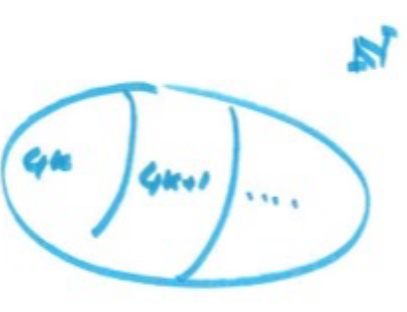
\includegraphics[scale=0.4]{images/rel_equi_quot.png}
    \caption{Insieme quoziente di $\equiv_4$}
\end{figure}

$\{[i]_4 : 0\leq i\leq 3\}$ è una partizione di $\mathbb{N}$ indotta dalla relazione
$\equiv_4$, tale per cui mi dia il rispettivo insieme quoziente (a volte impropriamente
chiamato $\mathbb{Z}_4$):
$$N / \equiv_4 \text{ }=\{[i]_4 : 0\leq i\leq 3\}=\mathbb{Z}_4$$

Adesso abbiamo in mano gli strumenti per definire in maniera molto più fine il concetto
di cardinalità.

\subsubsection{Cardinalità degli insiemi - II°}
Sia $\mathcal{U}$ (insieme universo) la classe di tutti gli insiemi,
definiamo la relazione $\sim\subseteq\mathcal{U}^2$ detta relazione
di \textit{equi numerosità} (hanno la stessa dimensione numerica), tra le coppie degli insiemi, se e solo se esiste
una \textbf{biezione} tra $A$ e $B$ (ovvero, se riesco ad esibire una funzione
iniettiva e suriettiva che va da $A$ in $B$).

Questa relazione tra insiemi è una relazione di equivalenza, poiché:
\begin{itemize}
    \item $\sim$ è riflessiva, se utilizzo la funzione identità $i_A$.
    \item $\sim$ è simmetrica, se esiste una biezione $A\rightarrow B$ allora
          esiste una biezione anche $B\rightarrow A$. Ovvero $A\sim B$ e $B\sim A$.
    \item $\sim$ è transitiva, se compongo funzioni biettive ottengo ancora una
          funzione biettiva.
\end{itemize}

Due insiemi che stanno in questa relazione vengono detti \textit{equi numerosi}. Ora
considerando l'insieme quoziente del nostro universo $\mathcal{U}$ rispetto alla
relazione di equi numerosità $\sim$ (quindi stesso numero di elementi in entrambi
i due insiemi), esso mi rappresenta il concetto di \textbf{cardinalità}
di un insieme.

\begin{figure}[H]
    \centering
    \includegraphics[scale=0.4]{images/insieme_quoziente_cardinalità.png}
    \caption{Insieme quoziente $\mathcal{U} / \sim$}
\end{figure}

Quindi spezzettando l'insieme $\mathcal{U}$ in classi di equivalenza
in questa classe di equivalenza ci sono tutti gli insiemi
che sono equi numerosi (seppur diversi).

Questo concetto permette di parlare in maniera molto precisa anche di
insiemi di cardinalità infinita.
Questi insiemi possono avere lo stesso numero
\newline
\newline
Per esempio, consideriamo $n\in\mathbb{N}^+$, si consideri l'insieme $J_n=\{1,2,,...,n\}$. Per questo
insieme è ovvio quale sia il concetto di cardinalità perchè è finito.

Allora diciamo che un insieme $A$ ha cardinalità \textbf{finita} se è equi
numeroso con $J_n$ (ovvero $A\sim J_n$) per un dato $n$ ed in quel caso scriviamo che $|A|=n$.

Quindi nella classe di equivalenza $J_1$ troviamo tutti gli insiemi con un
elemento, nella classe di equivalenza di $J_2$ troveremo tutti gli insiemi con due elementi, ecc.
\begin{figure}[H]
    \centering
    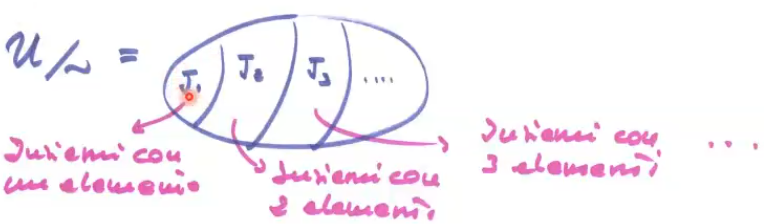
\includegraphics[scale=0.5]{images/U_insiemi_esemp_card2.png}
    \caption{Esempio $\mathcal{U}/\sim$ rispetto all'insieme $J_n$}
\end{figure}
Un insieme che non ha cardinalità si dice banalmente che ha cardinalità \textbf{infinità}. Fin qui abbiamo
parlato ancora di cardinalità finita, ma adesso faremo un esempio con cardinalità infinita.

\subsubsection{Insiemi numerabili}
$A$ si dice \textbf{numerabile} se è nella stessa classe di equivalenza dell'insieme dei numeri naturali
$\mathbb{N}$, ovvero se esiste una \textit{biezione} tra l'insieme $A$ e l'insieme $\mathbb{N}$.

Siccome stanno in relazione di equi numerosità
vuol dire che è presente una biezione fra i due elementi, quindi due elementi non possono collidere.

\begin{figure}[H]
    \centering
    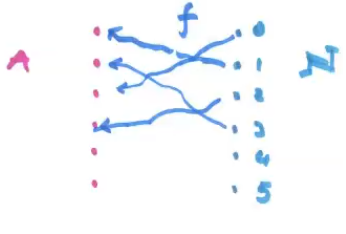
\includegraphics[scale=0.6]{images/A_numerabile_N.png}
    \caption{$A$ è un insieme numerabile}
\end{figure}

La presenza di questa biezione significa che come $A$ può essere \textbf{listato} con
$f(0),f(1),f(2),...$ su $\mathbb{N}$ senza perdere un elemento, anche l'insieme $\mathbb{N}$ può essere
listato a sua volta su $A$.

Alcuni esempi di insiemi numerabili:
\begin{itemize}
    \item I numeri pari $f(n)=2n$ , essi sembrerebbero la metà dei numeri naturali ma sono tanti quanto i numeri
          naturali perchè esiste questa biezione (vale anche per i dispari $f(n)=2n+1$).
    \item L'insieme $\mathbb{Z}$, possono essere presenti diverse funzioni, per esempio
          posso mappare i negativi sui numeri pari ed i positivi sui numeri dispari.
    \item L'insieme $\mathbb{Q}$, vedremo più avanti.
    \item L'insieme delle stringhe binarie che incominciano con $1$, ovvero $1\{0,1\}^*$,
          dove una funzione $f(n)=bin(n)$ è in grado di associare un numero naturale (utilizzando
          le potenze in posizione) ad una stringa binaria.
\end{itemize}

\subsubsection{Insiemi non numerabili}
Esistono degli insiemi che non sono listabili, dette in altre parole sono più fitti di $\mathbb{N}$,
è un altro tipo di categoria di infinito.
$$\mathbb{R}\text{ non è numerabile}$$
\paragraph{Dimostrazione}\mbox{}\\L'idea consiste nel dimostra per assurdo che non esiste una biezione
perchè sono presenti dei "buchi" tra le associazioni. Ordine della dimostrazione:
\begin{itemize}
    \item Dimostro che $\mathbb{R}\sim[0,1]$ (si dice che è \textit{isomorfo/equi numeroso} all'intervallo $[0,1]$),
          ovvero che è fitto quanto l'intervallo citato.
    \item Dimostro che $\mathbb{N}\nsim[0,1]$
    \item $\mathbb{R}\sim[0,1]\nsim\mathbb{N}\implies\mathbb{R}\nsim\mathbb{N}$
\end{itemize}

\paragraph{$R\sim[0,1]$}\mbox{}\\ \noindent Significa riuscire a rappresentare una funzione
che mappa gli elementi tra i due insiemi in maniera che sia suriettiva ed iniettiva.

Prima di tutto abbiamo una retta cartesiana con un origine fissata e che copre tutti i numeri reali.
Pongo l'intervallo $[0,1]$ in modo che si trovi in corrispondenza del punto mediano della retta $0$,
successivamente prendo un compasso punto il centro nel mediano dell'intervallo e traccio la
semi circonferenza rispetto alla metà dell'intervallo.

Gli elementi dell'insieme $\mathbb{R}$ vengono mappati tracciando una retta in direzione del punto
mediano di $[0,1]$, nel punto di intersezione si traccia la retta perpendicolare che interseca
l'intervallo ed in quel punto si trova il valore corrispondente. Si può fare lo stesso
in maniera opposta partendo da $[0,1]$, trovando l'intersezione si parte dal punto mediano
di quest'ultima e si attraversa l'intersezione toccando $\mathbb{R}$.

Questo dimostra che tutti i valori di $\mathbb{R}$ sono associabili
su $[0,1]$, quindi $\mathbb{R}\sim[0,1]$.
\pagebreak
\paragraph{$\mathbb{N}\nsim[0,1]$ (diagonalizzazione)}\mbox{}\\ Supponiamo per assurdo che $\mathbb{N}\sim[0,1]\implies[0,1]$,
ovvero che sia listabile in maniera esaustiva. Quindi quello che penso di fare consiste nel
costruire un elenco di numeri (tutti gli elementi iniziano con $0.$).
\[
    \begin{array}{ccccc}
        \underline{0.a_{11}} & 0.a_{12}             & 0.a_{13}             & 0.a_{14}             & ... \\
        0.a_{21}             & \underline{0.a_{22}} & 0.a_{23}             & 0.a_{24}             & ... \\
        0.a_{31}             & 0.a_{32}             & \underline{0.a_{33}} & 0.a_{34}             & ... \\
        0.a_{41}             & 0.a_{42}             & 0.a_{43}             & \underline{0.a_{44}} & ... \\
        ...                  & ...                  & ...                  & ...                  & ... \\
    \end{array}
\]
Per costruire un numero elusivo che non si trova in nessuno di questi elementi della lista,
vado a guardare le cifre sulla diagonale.

Per esempio costruiamo:
$$0.c_1c_2c_3c_4$$
L'$i$-esima cifra è fatta in questo modo
\[
    c_i=
    \begin{cases}
        a_{ii} + 1\text{ se }a_{ii} < 9 \\
        a_{ii} - 1\text{ se }a_{ii} = 9 \\
    \end{cases}
\]
Ora usando questa regola non riuscirò mai a costruire un numero tra quelli elencati,
questo perchè ovviamente cambio le cifre.
Il numero $0.c_1c_2...\in[0,1]$, ma non appartiene nelle liste poiché:
\begin{itemize}
    \item Differisce dal primo perché $c_1\neq a_{11}$
    \item Differisce dal secondo perché $c_2\neq a_{22}$
    \item Differisce da qualunque numero presente sulla diagonale
\end{itemize}
Quindi la lista non è esaustiva $\implies \mathbb{N}\nsim[0,1]$.

\paragraph{Conclusione}\mbox{}\\
$$\mathbb{R}\sim[0,1]\nsim\implies\mathbb{R}\nsim\mathbb{N}$$
\begin{itemize}
    \item $\mathbb{R}$ non è numerabile.
    \item Esso è più \textit{"fitto"} di $\mathbb{N}$.
    \item Qualsiasi tentativo di listare anche solo un segmento non è esaustivo.
    \item $\mathbb{R}$ è un insieme \textbf{continuo}, e tutti gli insiemi equi numerosi
          $\mathbb{R}$ si dicono continui.
    \item Altri esempi di insiemi non numerabili:
\end{itemize}
%da capire ancora.

\subsubsection{Insieme delle parti di $\mathbb{N}$}
$$P(\mathbb{N})=2^{\mathbb{N}} = \{\text{sottoinsiemi di }\mathbb{N}\}\nsim\mathbb{N}$$
Posso rappresentare i sotto insiemi di $\mathbb{N}$ utilizzando un \textbf{vettore caratteristico}
$A\subseteq\mathbb{N}$.
\[
    \mathbb{N}\rightarrow
    \begin{array}{cccccccc}
        0 & 1 & 2 & 3 & 4 & 5 & 6 & ... \\
    \end{array}
\]
\[
    A\rightarrow
    \begin{array}{cccccccc}
        0 & 1 & 1 & 0 & 1 & 1 & 0 & ... \\
    \end{array}
\]
Questo è un vettore di booleani (o bit) che mette segnala la presenza degli elementi dell'insieme
dei numeri naturali in $A$, quindi $0$ quando l'elemento corrispondente di $\mathbb{N}$ non
appartiene ad $A$, e viceversa $1$ se appartiene.
%terminare
\subsection{Insieme non numberabile $\mathbb{N}^{\mathbb{N}}$}




\end{document}